\documentclass{article}
\usepackage{titlesec}

%Paquetes
\usepackage[left=4cm, right=4cm]{geometry}
\usepackage{fancyhdr}
\usepackage{palatino}%Fuente
 \usepackage{eulervm}%Fuente
\usepackage{graphicx}%Imágenes
\usepackage{float}%Imágenes
\usepackage{subcaption}%Imágenes
\usepackage{enumitem}%Listas
\usepackage{parskip}%Espacio entre párrafos
\usepackage{multicol}
\usepackage{amsthm,thmtools,xcolor}
\usepackage{amssymb}%Mate
\usepackage{amsmath}%Mate
\usepackage{tikz}%Mate (diagramas)
\usepackage{dutchcal}
\usepackage{tikz-cd}
\usepackage{xcolor}
\definecolor{blue-violet}{rgb}{0.54, 0.17, 0.89}
\usetikzlibrary{%
	matrix,%
	calc,%
	arrows,%
	shapes,
	decorations.markings,backgrounds,calc,intersections
}
\usepackage[bookmarks,bookmarksopen,bookmarksdepth=3]{hyperref}%Links a lugares en el texto
\hypersetup{%colores
	colorlinks=true,
	urlcolor=blue,
	linkcolor=magenta,
	citecolor=blue,
	filecolor=blue,
	urlbordercolor=white,
	linkbordercolor=white,
	citebordercolor=white,
	filebordercolor=white
}
\usepackage{cleveref}
\Crefname{exercise}{Exercise}{Exercises}


\makeatletter %Hide section number
\def\@seccntformat#1{%
	\expandafter\ifx\csname c@#1\endcsname\c@section\else
	\csname the#1\endcsname\quad
	\fi}
\makeatother
\usepackage{sectsty}
\sectionfont{\fontsize{17}{20}\selectfont}


%Referencias
%\usepackage[style=authortitle,backend=bibtex]{biblatex}
%\addbibresource{exercises.bib}

\definecolor{blue-violet}{rgb}{0.54, 0.17, 0.89}
\definecolor{azure}{rgb}{0.0, 0.5, 1.0}
\definecolor{green(ncs)}{rgb}{0.0, 0.62, 0.42}
\definecolor{forestgreen}{rgb}{0.13, 0.55, 0.13}
\definecolor{limegreen}{rgb}{0.2, 0.8, 0.2}
\definecolor{palatinateblue}{rgb}{0.15, 0.23, 0.89}
\definecolor{trueblue}{rgb}{0.0, 0.45, 0.81}
\definecolor{goldenyellow}{rgb}{1.0, 0.87, 0.0}
\definecolor{fashionfuchsia}{rgb}{0.96, 0.0, 0.63}
\definecolor{brightcerulean}{rgb}{0.11, 0.67, 0.84}
\definecolor{jonquil}{rgb}{0.98, 0.85, 0.37}
\definecolor{lavendermagenta}{rgb}{0.93, 0.51, 0.93}
\definecolor{peru}{rgb}{0.8, 0.52, 0.25}
\definecolor{persimmon}{rgb}{0.93, 0.35, 0.0}
\definecolor{persianred}{rgb}{0.8, 0.2, 0.2}
\definecolor{persianblue}{rgb}{0.11, 0.22, 0.73}
\definecolor{persiangreen}{rgb}{0.0, 0.65, 0.58}
\definecolor{persianyellow}{rgb}{0.9, 0.89, 0.0}

%\theoremstyle{definition}

\declaretheoremstyle[headfont=\color{trueblue}\normalfont\bfseries,]{colored1}
\declaretheoremstyle[headfont=\color{forestgreen}\normalfont\bfseries,]{colored2}
\declaretheoremstyle[headfont=\color{peru}\normalfont\bfseries,]{colored3}
\declaretheoremstyle[headfont=\color{persiangreen}\normalfont\bfseries,]{colored4}
\declaretheoremstyle[headfont=\color{brightcerulean}\normalfont\bfseries,]{colored5}
\declaretheoremstyle[headfont=\color{lavendermagenta}\normalfont\bfseries,]{colored6}
\declaretheoremstyle[headfont=\color{blue-violet}\normalfont\bfseries,]{colored7}
\declaretheoremstyle[headfont=\color{green(ncs)}\normalfont\bfseries,]{colored8}
\declaretheoremstyle[headfont=\color{peru}\normalfont\bfseries,]{colored9}
\declaretheoremstyle[headfont=\color{persiangreen}\normalfont\bfseries,]{colored10}

\declaretheorem[style=colored1,numberwithin=section,name=Theorem]{thm}
\declaretheorem[style=colored2,numberwithin=section,numberlike=thm,name=Proposition]{prop}
\declaretheorem[style=colored3,numberwithin=section,numberlike=thm,name=Lemma]{lemma}
\declaretheorem[style=colored4,numberwithin=section,numberlike=thm,name=Corollary]{coro}
\declaretheorem[style=colored5,numbered=no,name=Example]{example}
\declaretheorem[style=colored5,numbered=no,name=Examples]{exemplos}
\declaretheorem[style=colored6,numberwithin=section,name=Exercise]{exercise}
\declaretheorem[style=colored7,numberwithin=section,name=Remark]{remark}
\declaretheorem[style=colored9,numbered=no,name=Claim]{claim}
\declaretheorem[style=colored8,numbered=no,name=Definition]{defn}
\declaretheorem[style=colored10,numbered=no,name=Question]{question}

\numberwithin{equation}{section}

\newcommand{\R}{\mathbb{R}}
\newcommand{\Z}{\mathbb{Z}}
\newcommand{\N}{\mathbb{N}}
\newcommand{\C}{\mathbb{C}}
\newcommand{\Q}{\mathbb{Q}}
\newcommand{\D}{\mathbb{D}}
\renewcommand{\P}{\mathbb{P}}
\newcommand{\Ac}{\mathcal{A}}
\newcommand{\Bc}{\mathcal{B}}
\newcommand{\Cc}{\mathcal{C}}
\newcommand{\Dc}{\mathcal{D}}
\newcommand{\Ec}{\mathcal{E}}
\newcommand{\Fc}{\mathcal{F}}
\newcommand{\Gc}{\mathcal{G}}
\newcommand{\Lc}{\mathcal{L}}
\newcommand{\Oc}{\mathcal{O}}
\newcommand{\Qc}{\mathcal{Q}}
\newcommand{\Sc}{\mathcal{S}}
\newcommand{\Wc}{\mathcal{W}}
\newcommand{\mf}{\mathfrak{m}}

\renewcommand{\Im}{\operatorname{Im}}

\DeclareMathOperator{\img}{img}
\DeclareMathOperator{\Arg}{Arg}
\DeclareMathOperator{\id}{id}
\DeclareMathOperator{\Alt}{Alt}
\DeclareMathOperator{\sgn}{sgn}
\DeclareMathOperator{\supp}{supp}
\DeclareMathOperator{\Int}{Int}
\DeclareMathOperator{\Ob}{Ob}
\DeclareMathOperator{\Mor}{Mor}
\DeclareMathOperator{\Top}{Top}
\DeclareMathOperator{\CGWH}{CGWH}
\DeclareMathOperator{\Hom}{Hom}
\DeclareMathOperator{\Map}{Map}
\DeclareMathOperator{\Tot}{Tot}
\DeclareMathOperator{\Vect}{Vect}
\DeclareMathOperator{\VectBund}{VectBund}
\DeclareMathOperator{\Open}{Open}
\DeclareMathOperator{\Ring}{Ring}
\DeclareMathOperator{\Set}{Set}

\pagestyle{empty}
\fancyhf{}
\cfoot{\thepage}
\rhead{Daniel González Casanova Azuela}
\lhead{Complex manifolds in dimension 1}
\begin{document}

\section{Home Assignment 1: holomorphic functions}
\thispagestyle{fancy}


\begin{exercise}\label{exercise:1}
	Let $f$ be a holomorphic function on a disk $\Delta$. Prove that the zero set $Z_f$ of $f$ is discrete in $\Delta$.
\end{exercise}
\begin{proof}
	
	
	Suppose there exists $z_0\in Z_f\cap Z_f'\cap \Delta$, a zero of $f$ in $\Delta$ that is also an accumulation point of $Z_f$. Then there is a sequence $(z_k)\subset Z_f$ that converges to $z_0$. So $f\equiv0$ in $(z_k)\cup\{z_0\}$, and by the identity principle $f\equiv0$ in $\Delta$.
\end{proof}

\begin{exercise}\label{exercise:2}
	Let $P(t)$ be a polynomial. Prove that $f(z) = z - \frac{P (z)}{P'(z)}$ is holomorphic
	 in a neighbourhood of any $\alpha$ which is a root of $P(t)$. Prove that $f(\alpha) = \alpha$ and $|f'(\alpha)| < 1$.
\end{exercise}
\begin{proof}
	We have that
	\[P(z)=Q(z)(z-\alpha)^k\]
	where $Q(\alpha)\neq0$. So
	\begin{align*}
		P'(z)&=Q'(z)(z-\alpha)^k+kQ(z)(k-\alpha)^{k-1}\\
		&=(z-\alpha)^{k-1}(Q'(z)(z-\alpha)+kQ(z)),
	\end{align*}
	and then the quotient is
	\[\frac{P(z)}{P'(z)}=(z-\alpha)\frac{Q(z)}{Q'(z)(z-\alpha)+kQ(z)}\]
	which is well-defined in a neighbourhood of $\alpha$ where there are no other roots of $P(z)$ (we may use \cref{exercise:1}). Thus $f$ is holomorphic near $\alpha$.
	
	It is clear that $f(\alpha)=\alpha$.
	
	{\color{blue-violet} I couldn't really prove that $|f'(\alpha)|<1$.
	
	\textbf{Here's some ideas}:
	
	Notice that
	\[f'(z)=1-\frac{P'(z)^2-P''(z)P(z)}{P'(z)^2}=\frac{P''(z)P(z)}{P'(z)^2}.\]
	
	Now suppose that
	\[P(z)
	%=\sum_{n=0}^da_nz^n
	=a_0+a_1z+a_2z^2+a_3z^3+\ldots+a_nz^n.\]
	Then
	\begin{align*}
		P'(z)&=a_1+2a_2z+3a_3z^2\ldots+na_nz^{n-1}\\
		P''(z)&=2a_2+3\cdot2a_3z+\ldots+n\cdot(n-1)a_nz^{n-2}
	\end{align*}
%	So
%	\begin{align*}
%		\frac{P(z)}{P'(z)}&=\frac{a_0+a_1z+a_2z^2+\ldots+a_nz^n}{a_1+2a_2z+\ldots+na_nz^{n-1}}\\
%		&=\frac{a_0+a_1z+\ldots+a_{n-1}z^{n-1}}{a_1+2a_2z+\ldots+na_nz^{n-1}}+z\frac{a_nz^{n-1}}{a_1+2a_2z+\ldots+na_nz^{n-1}}
%	\end{align*}
	and then …?}
\end{proof}

\begin{exercise}
	Let $f(z)$ be a non-constant holomorphic function on a disk $\Delta$. Prove that there exist $t, s \in]0, 1]$ such that the function $f (tz) - f (sz)$ has no zeros when $|z| = 1$.
\end{exercise}
\begin{proof}
	\iffalse If for all $t,s\in]0,1]$ there is $z$ of norm one such that $f(tz)=f(sz)$, means that for every pair of concentric circles within $\Delta$ there is a direction such that $f$ has the same value in those two circles in that direction. We obtain a set of directions at which $f$ is not injective.\fi
	
	
	 By contradiction, suppose that for all $t,s\in]0,1]$ there is $z$ of norm 1 such that $f(tz)=f(sz)$. For $s=1$ and $t_n=1/n$ with $n\in \N$, there exists $z_n$ of norm 1 such that $f(z_n/n)=f(z_n)$. Denoting $z_0=\lim_nz_n$, we get by continuity that $f(0)=f(z_0)$.
	 
	 By a similar argument but now varying $s$ in $]0,1]$, we obtain numbers $z_{0,s}$ of norm $s$ such that $f(0)=f(z_{0,s})$. But then $f\equiv f(0)$ in a infinite set within a compact set, which must have an accumulation point, so $f$ is constant.
	 
	 %But $f$ cannot attain a maximum of minimum value inside $\Delta$, so $f(z_0)$ cannot be a maximum or minimum. \textbf{Idea:} show that any point in $\partial\Delta$ 
	 
	% By exercise 1.4, $f(z_0)=\frac{1}{\pi}\int_\Delta f=\frac{1}{2\pi}\int_{\partial\Delta}f$.
\end{proof}

\begin{exercise}
	Prove that if $f$ is holomorphic on the unit disk $\Delta$ and continuous on $\partial\Delta$, then $\frac{1}{\pi}\int_\Delta f=f(0)$.
\end{exercise}
\begin{proof}
	We know that the real and imaginary parts of $f$ are harmonic functions. By the mean value property
	\[f(0)=u(0)+\sqrt{-1}v(0)=\frac{1}{\pi}\left(\int_\Delta u+\sqrt{-1}\int_\Delta v\right),\]
	where $f=u+\sqrt{-1}v$, using that the area of the unit disk is $\pi$.
\end{proof}

\begin{exercise}
	Prove that any holomorphic map from $\C\backslash0$ to a disk $\Delta$ is constant.
\end{exercise}
\begin{proof}[Solution]
	By Riemann's criterion of removable singularities, $0$ is a removable singularity of $f$ since $f$ is bounded. Thus there is a holomorphic function extending $f$ to all of $\C$, which must be constant by Liouville's theorem, making $f$ constant as well.
\end{proof}

\begin{exercise}
	Prove that any holomorphic function on a disk $\Delta$ which is continuous on its boundary $\partial\Delta$ and takes real values on $\partial\Delta$ is constant, or find a counterexample.
\end{exercise}
\begin{proof}[Solution]
	If we had $f$ holomorphic on an open neighbourhood of $\Delta$, then we can borrow this reasoning from \href{https://math.stackexchange.com/questions/3482976/holomorphic-function-with-real-values-on-boundary}{StackExchange}:
	\begin{quote}
		$\Im(f)$ is harmonic, and 0 on $\partial\Delta$. If it were not identically 0, it would have a maximum or minimum in $\Delta$, and that is impossible.
	\end{quote}
	This would mean that $f$ is a real-valued function, so its derivative must be zero.
	
	But in fact, $f$ can be holomorphically extended by Schwarz reflection principle, which states that any function that is holomorphic on the upper half plane and real-valued on the real axis is holomorphically extendable to the whole plane. So we only need to precompose $f$ with some holomorphic function taking the upper half-plane to our given disk (and then translate and resize).
	
	The Cayley transform $z\mapsto \frac{z-i}{z+i}$ has such an action with respect to the unit disk:
	
	\begin{figure}[H]
		\centering
		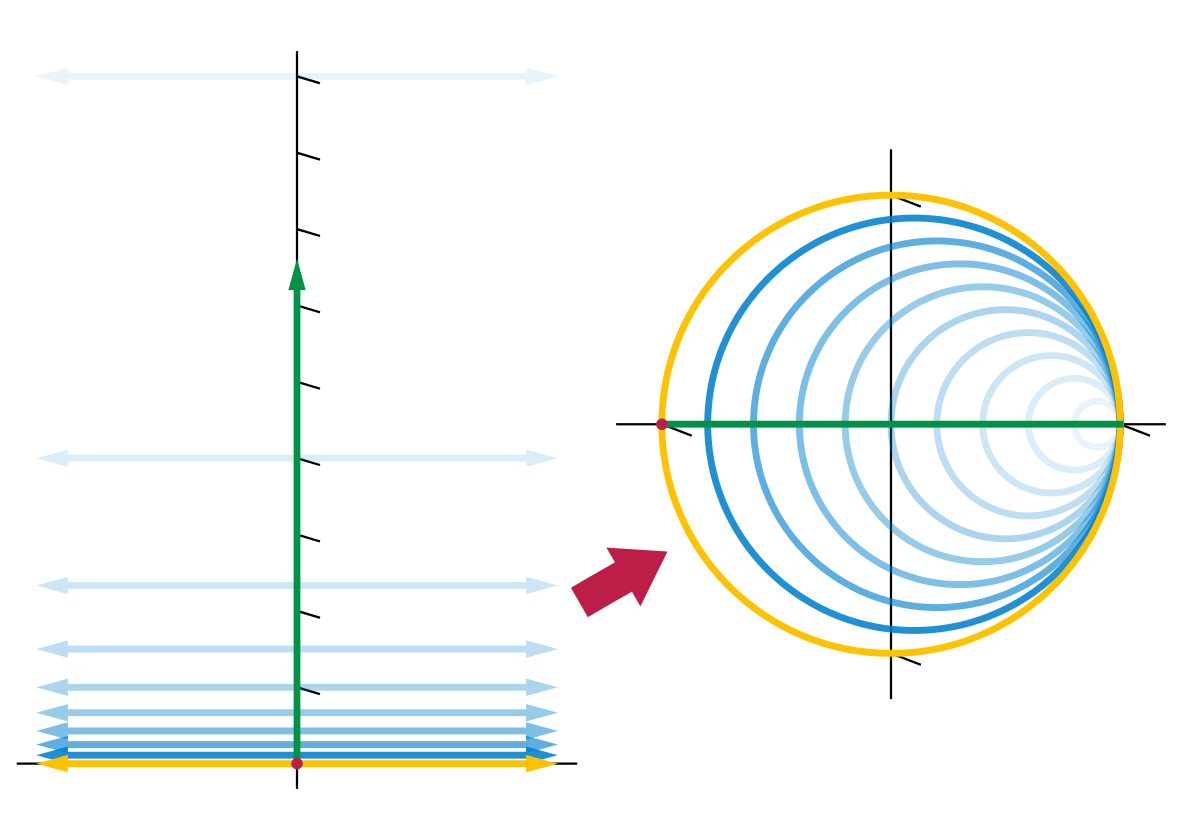
\includegraphics[width=0.7\linewidth]{fig1}
		\label{fig:fig1}
	\end{figure}	
\end{proof}
\end{document}